\section{Finding a real zero from finitely many noisy samples}
\label{sec:root-realizer}

A rational polynomial permits an exact sign test at each rational midpoint.
The repository's \texttt{Analysis.PolynomialBisection} uses this fact,
and \texttt{PolynomialRootName} constructs a regular root name from the
nested brackets. Its \texttt{PolynomialRootUniqueness} uses a positive
divided-difference bound to compare independently obtained names.
For a polynomial with \emph{named real coefficients} the midpoint value
may itself be an undecidable zero. We give a bounded replacement for
this sign test. It works at repeated roots and in intervals containing
several roots.

\subsection{What a modulus alone buys}

Put $e_k=2^{-k}$. A rational evaluator $E(x,p)$ on $[0,1]$ has error
$e_p$ for the continuous function $f$ it presents. Its continuity modulus
$\mu$ guarantees $|f(x)-f(y)|\le e_j$ whenever $|x-y|\le e_{\mu(j)}$.
These semantic inequalities abbreviate the rational bounds
$|E(x,p)-E(y,q)|\le e_p+e_j+e_q$ on qualifying pairs, together with
$|E(x,p)-E(x,q)|\le e_p+e_q$. A weak initial bracket means
$E(0,p)\le e_p$ and $E(1,p)\ge-e_p$ for all $p$. Evaluators and moduli
are fixed PR programs, possibly with number parameters.

\paragraph{Approximate intermediate values.}
At demand $k$, set $p=k+2$ and start with $[a,b]=[0,1]$. For at most
$\mu(k+1)$ steps sample $v=E((a+b)/2,p)$. If $|v|\le e_p$, return
the midpoint. If $v>e_p$, replace $b$ by the midpoint. Otherwise
$v<-e_p$, so replace $a$. At exhaustion return the remaining midpoint.
An early answer has residual at most $2e_p$. Each update preserves
$f(a)\le0\le f(b)$. At exhaustion the bracket has width at most
$e_{\mu(k+1)}$, so its midpoint value is both at most $e_{k+1}$ above
the left endpoint value and at most $e_{k+1}$ below the right endpoint
value. The residual is therefore at most $e_{k+1}$ in both cases.
Internally the output $z$ satisfies
$|E(z,q)|\le e_q+e_{k+1}$ for every $q$. To obtain this bound fix $q$ before induction,
using the endpoint bounds at an arbitrary auxiliary precision $t$.
For example an exhausted bracket gives
$E(z,q)\le e_q+e_{k+1}+2e_t$ for every $t$. If the claimed rational
upper bound failed, its positive rational excess would give a bounded
choice of $t$ with $2e_t$ smaller than that excess (the denominator
plus two suffices for a reduced positive rational). The lower bound
follows the same way. There are at most
$\mu(k+1)$ evaluator calls, compared with $2^{\mu(k+1)}+1$ points in
the full uniform mesh. This is a query count. The cost of a call depends
on its provider. Frank's constructive approximate IVT gives an existence
result even under pointwise continuity. Here the supplied modulus serves
to calculate the finite stopping budget.\footnote{M. Frank,
\emph{Interpolating Between Choices for the Approximate Intermediate
Value Theorem}, \href{https://arxiv.org/abs/1701.02227}{arXiv:1701.02227}.}

\paragraph{A finite-use obstruction.}
No uniform oracle algorithm can, from these same data, return a regular
name of an exact zero for every input. Consider
\[
 g(x)=\min(x-1/3,0)+\max(x-2/3,0).
\]
This function and all vertical translates are $1$-Lipschitz. Run a
hypothetical algorithm on the exact rational evaluator for $g$ to obtain
a root approximation of error at most $1/16$. Let $b$ bound the
precisions of its finitely many requests. Choose a positive dyadic
$c<\min(1/12,e_b)$. Give the two inputs $g+c$ and $g-c$ evaluators
that return $g(x)$ at precisions up to $b$ and exact values thereafter.
They have the same Lipschitz modulus and each has the required strict
endpoint crossing. The two runs have the same transcript by deterministic
replay. Their unique roots are $1/3-c$ and $2/3+c$. They are more than
$1/3$ apart, so no common answer works. This is a representation-level
impossibility even for PR families fed through their evaluators. The
argument does not concern algorithms given extra symbolic syntax. It is
the root analogue of the repository's
\texttt{Foundations.FiniteUseSignObstruction}.

\subsection{A local certificate for coherent brackets}

At stage $n$, a certificate on $I=[a,b]$ consists of a rational
$z\in[a+(b-a)/3,b-(b-a)/3]$ and a precision $p$ with
$|E(z,p)|>e_p$. A fixed PR producer of these data suffices. Retain
$[a,z]$ for a positive value and $[z,b]$ for a negative value.
Each interval is nested, retains the weak bracket, and has length
between one third and two thirds of its predecessor. Let $x_k$ be
the midpoint after $2k$ stages. Since $(2/3)^2<1/2$,
\[
    |I_{2k}|\le e_k,\qquad
    |x_l-x_k|\le e_k/2\quad(l\ge k).
\]
All runs use the same stage-indexed producer and tie rule, so they agree
on their shared prefix. This defines a regular name. Given output
residual demand $j$, use any $k\ge\mu(j)$ in the endpoint estimate
above to obtain $|f(x_k)|\le e_j$. Continuity yields $f(x)=0$ for
the named limit $x$. This proves a root relation. Different presentations
of a polynomial with several roots may produce different valid roots.
For a unique root all such outputs agree. No compatibility between
independently chosen approximate zeros is assumed.

\subsection{Producing the certificate for a monic polynomial}

\paragraph{Polynomial crossing theorem.}
Let $d\ge1$ and
$P(t)=t^d+\sum_{i<d}c_it^i$, where $c_i$ has a rational name $C(i,s)$
of error $e_s$. Suppose $P(0)\le0\le P(1)$. Then one uniform
PR algorithm in the degree and numerical parameters of the fixed
coefficient provider returns a regular name of a real zero in $[0,1]$.
It uses $2kd$ coefficient queries for position demand $k$, including
in the presence of multiple roots. For a model charging one query per
coefficient table, the count is $2k$.

\paragraph{A rational observation that forces a sign.}
For a rational monic $Q$ of degree $d$, step $h>0$, and starting point
$u$, the $d$th forward difference of $Q$ is the constant $d!h^d$.
Indeed $Q(t+h)-Q(t)$ has degree $d-1$ and leading coefficient $dh$,
by the binomial identity. Repetition gives the claimed constant.
If $M=\max_{0\le i\le d}|Q(u+ih)|$, one difference row has entries
bounded by $2M$ by the triangle inequality. Repeating gives
\[
  d!h^d\ \le\ 2^d M.                                      \tag{R1}
\]
A bounded rational scan therefore finds a large value, even when
particular probes evaluate to zero. The forward differences are used
in the proof only.

\paragraph{Precision and cost.}
Let $w=b-a$ at stage $n$, set $u=a+w/3$, $h=w/(3d)$, and use
the $d+1$ points $u+ih$ in the middle third. Write
$\ell(v)=\min\{r\le v:2^r\ge v\}$ for positive integer $v$.
Use
\[
   p_n=d\bigl(\ell(6d)+2n\bigr)+3,\qquad s_n=p_n+\ell(d).
\]
Read each of the $d$ coefficients once at $s_n$ and form the monic
rational polynomial $Q_n$ with those coefficients. On $[0,1]$,
$|P-Q_n|\le d e_{s_n}\le e_{p_n}$. Because $w\ge3^{-n}$,
\[
   \frac{d!h^d}{2^d}\ \ge\ (6d\,3^n)^{-d}\ \ge\ 8e_{p_n}.
\]
Choose the least node index attaining the maximum in (R1). Its
$Q_n$-value has magnitude at least $8e_{p_n}$, so its sign certifies
the sign of $P$. This produces the local certificate at every stage
from the coefficients alone. Induction gives the nested intervals above.
Any $2k$-stage run evaluates at most $2k(d+1)$ rational polynomial
values by Horner's rule. For $k\ge1$ the greatest coefficient precision read is $s_{2k-1}$. The Horner evaluations cost $O(kd^2)$ rational arithmetic operations, with growing operand sizes. The stage precision depends only on $n,d$.
Reusing the same stage table at its $d+1$ nodes is valid because it
defines one rational monic polynomial. Replacing all past tables by
a finer one when computing a new output demand could change earlier
maximizers and lose this prefix guarantee.

\paragraph{Adequacy in first-order arithmetic.}
For clarity let $P_s$ denote the rational polynomial with coefficients
$C(i,s)$. At rational $v\in[0,1]$ the finite coefficient loop gives
$|P_s(v)-P_t(v)|\le d(e_s+e_t)$. The weak bracket input is the pair of
universally indexed estimates $P_s(0)\le de_s$ and
$P_s(1)\ge-de_s$. Fix $s$ as a parameter. At each selected positive
node, $Q_n(z)\ge8e_{p_n}>de_{s_n}$ implies $P_s(z)\ge-de_s$ by
cross-precision comparison. At a negative node the reverse inequality
holds. Thus $P_s(a)\le de_s$, $P_s(b)\ge-de_s$ are quantifier-free
iteration invariants. For $s\ge0$ the coefficients of $P_s$ have
absolute value at most $|C(i,0)|+2$ by regularity. A rational upper
bound for their common Lipschitz constants is
\[
   H=d+\sum_{i<d}i(|C(i,0)|+2),
\]
using $|v^i-t^i|\le i|v-t|$ on the unit interval (expand the
difference of powers). The two endpoint inequalities therefore give
\[
   |P_s(x_k)|\le de_s+He_k/2.                             \tag{R2}
\]
For requested residual error $e_j$, taking
$s=j+2+\ell(d)$ and $k=j+2+\ell(\max(1,\lceil H\rceil))$
suffices. This proves the represented zero statement entirely by
rational observations. Degrees, rows of differences, and all scans
are numbers or finite lists. For a uniform-degree proof encode the
coefficient transformation for each difference row by the binomial
formula and reflect the bounded conjunction of its coefficient
equalities into one Boolean. The leading-term law and the factor two
row bound then use quantifier-free induction on the row index.
The result asks for neither the intervening zeros nor the multiplicities.

\paragraph{Odd degree without a supplied bracket.}
For odd $d$, let $S=\sum_{i<d} (|C(i,0)|+1)$ and $R=2+\lceil S\rceil$.
At $\pm R$ all lower terms together have size at most
$S R^{d-1}<R^d$. The monic polynomial
$T(t)=P(2Rt-R)/(2R)^d$ thus has the unit-interval bracket.
Binomial expansion gives its coefficient of $t^j$ as a fixed finite
linear combination of the $c_i$ and an exact contribution from the
leading monomial. For $j\le i<d$ the absolute multiplier is
$\binom{i}{j}(2R)^jR^{i-j}/(2R)^d\le 2^d$. Hence one may compute each
new coefficient to error $e_p$ by reading the old ones at
$p+d+\ell(d)$. Apply the theorem and map the resulting name back
by $t\mapsto2Rt-R$, shifting its position demand by $\ell(2R)$.
This gives a PR multivalued realizer for a real root of any named monic
odd-degree polynomial with a fixed PR coefficient family. The stated
$2kd$ query count applies to the normalized unit-interval input.

\paragraph{Which root is returned?}
For $P(x)=(x-1/4)(x-1/2)(x-3/4)$ the first-stage absolute values
are maximal at $1/3$ and $2/3$, and the signed values there are
$5/864$ and $-5/864$. The inner two nodes have magnitude
$77/23328<5/864$. Perturb just the constant coefficient table by
$+e_s$ at each precision $s$, or by $-e_s$. Both are names of the
same coefficient. The first choice retains $[0,1/3]$ at the first
stage, and the second retains $[2/3,1]$. Only one zero lies in each
retained bracket, so the resulting roots are $1/4$ and $3/4$.
The multivalued specification thus matters even for one rational
polynomial with simple roots. The supplied tests also check a triple
root and $(x-1/2)^2(x^3-\sqrt{2}/4)$, whose coefficient provider
uses integer square roots for rational enclosures.

\begin{figure}[htbp]
\centering
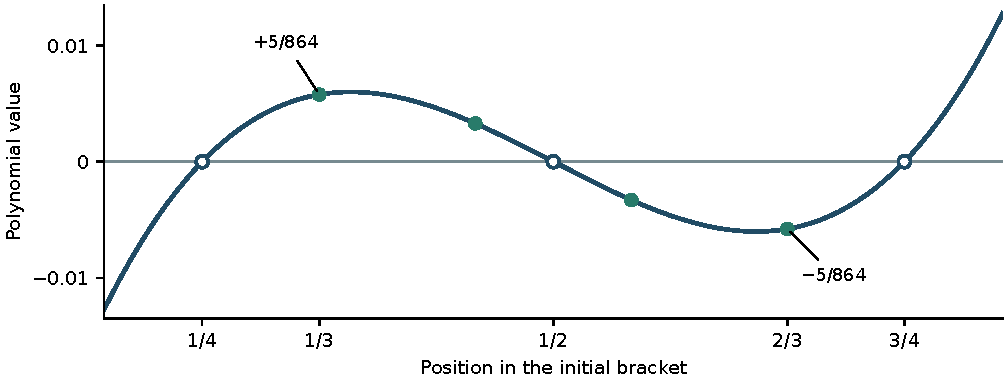
\includegraphics[width=.8\linewidth]{figures/root-probes.pdf}
\caption{Four middle-third probes of the cubic with roots at $1/4$, $1/2$ and $3/4$. The outer probes tie for largest magnitude, with opposite signs. Tiny admissible perturbations of the coefficient observations can break the tie in either direction.}
\end{figure}

\paragraph{Lean boundary.}
In \texttt{Root.lean}, \texttt{best} is the first maximizing index,
\texttt{difference\_bound} proves the $2^d$ estimate for successive
differences, and \texttt{monic\_peak} proves (R1) for an arbitrary
rational monic polynomial, degree, origin, and positive rational step.
It applies mathlib's factorial identity to $Q(u+hX)$ and uses that
polynomial's computed leading coefficient $h^d$. The lemma
\texttt{positive\_endpoint} is the sign-transport inequality for a
fixed target precision. These are checked ambient Lean theorems.
For the object-language endpoint encode the state as a rational endpoint
pair and let the PR step build a coefficient table, evaluate by Horner,
scan for the first maximum, and choose the subinterval by rational sign.
Use (R1)'s finite row proof above for the compiled difference-table
lemma, and (R2)'s two rational inequalities as the endpoint invariant.
Instantiate it twice for the desired endpoint precision and the final
sample comparison. Induct separately on a finite extension length for
nesting. These latter proof objects and the deep polynomial table
derivation remain to be constructed. The existing object proofs
\texttt{PolynomialBisection} and \texttt{PolynomialRootName} provide
the signed-rational bracket and regularity patterns at the pinned
revision.
